\section{Introduction}
\label{sec:intro}

% story line

% 1. The research question: with today’s sim tech, how much visual generalization can be obtained by single-task policies?
    % tairan: why is door opening hard? table top manipulation is easy, door-opening is a long-lasting problem cannot be solved by current approach; teleoperation does not give good result, sim2real is the only way to go for humanoid opening door (consider citing DARPA challenge paper, previous paper only on wheeled robot)
    % describe clearly why it is hard

    % why do we need to solve this task: a must-have skill for wide humanoid deployment
    % "humanoid is justified via being close to human form and suitable for human environment, yet they cannot open doors yet which is a basic skill"
%     1. There has been recent work on RGB Sim2Real (e.g. DextrAH-RGB)
%     2. Pick a hard task: humanoid loco manipulation (opening doors)
%     3. Previous door-opening paper are simplified
%         1.  Relies on depth or hand-crafted features and primitives on wheeled base (DoorBot, Haoyu’s paper https://arxiv.org/pdf/2401.14403).
%         2. Relies on simplified contact (hook) and ground truth localization  ([Marco Hutter paper](https://arxiv.org/pdf/2409.04882))
%     4. Mitigate partial observability in teacher-student distillation
%         1. One advantage of sim is to use privileged info in teacher
%         2. Partial observability was previously handled by adaptation structure like RMA
%         3. We need a new way to mitigate the perception gap in teacher
%         4. The student should learn to make up for missing information during finetuning
% 2. The underlying importance: if we find the right sim randomization receipe, we can find a cheap way to scale robot learning in sim
% 3. The approach: we design a controlled sim2real pipeline that isolates the effect of different components in RGB sim2real
%     1. Procedural generation pipeline for articulated objects
%     2. Teacher training with reset based exploration encouragement
%         1. The cost of being in a new stage and don’t know what to do could be high and may discourage the agent from entering said new stage
%         2. Solution: use a circular buffer to cache and force the agent to be resetted to the new stage directly
%     3. Fine-tune with GRPO
%         1. Example: the policy learns to optimize for making sure the handle is in the view of the camera
% 4. The novelty: we incorporate novel designs previous undiscussed in humanoid whole-body controll literature
%     1. Reset based exploration encouragement
%     2. Incremental set point action space
%     3. GRPO-based finetuning to mitigate partial observability
% 5. The result: robust open-world deployment of a humanoid door-opening policy
%     1. Ablation A: training speed with/without staged based exploration
%     2. Ablation B: training with absolute / relative / incremental set point action space
%     3. Ablation C: training with no / few / full visual feature randomization
%     4. Ablation D: training without door physical property randomization
%     5. Performance comparison: average time to complete compared with human teleop

\begin{figure*}[t]
    \centering
    \includegraphics[width=\linewidth]{figs/drafts/fig_result.pdf}
    \caption{Real-world generalization of \method{}. Top: diverse handle visuals and physical shapes. Middle: diverse wall panel visuals. Bottom: pushing and pulling open doors naturalistically.}
    \label{fig:result}
\end{figure*}

\textit{The reality of robotics is that humanoid kung fu and backflips are solved before they can open doors using only RGB vision.}

% Seemingly a trivial task, door opening stress tests every aspect of a humanoid robot system. The policy must identify the grasping location with a constantly vibrating camerea feed, rotate the handle against the spring-loaded force, swirl the door panel compliantly following its circular trajectory, while maintaining balance under the resistance from the hinge. These tightly coupled perception–action demands make door opening a strong indicator of real-world robustness and autonomy, particularly for humanoids intended to operate in everyday environments.

% Existing door-opening systems typically fall short of this goal. Many rely on depth sensing, hand-crafted features, or hard-coded primitives on wheeled platforms~\cite{calvert2025behavior, xiong2024adaptive, weng2025hdmi}. Others simplify contact mechanics with hooks or require accurate object localization~\cite{traverse-doors-2025}. Several DARPA-Robotics-Challenge–era systems~\cite{oh2017technical} depended on extensive scripting and operator intervention, and more recent teleoperation-heavy pipelines~\cite{lee2025stageact} remain labor-intensive and brittle. However, these methods cannot yield an autonomous policy capable of handling the wide variety of doors encountered in everyday human environments.

% Recent advances in hardware and simulation make it feasible to tackle door opening via sim-to-real. Although sim-to-real algorithms have shown strong results in humanoid locomotion~\cite{zhuang2024humanoid,wang2025beamdojo,long2025learning,ren2025vb,xue2025leverb, ben2025homie}, motion tracking~\cite{liao2025beyondmimic,luo2025sonic,he2025asap}, and manipulation~\cite{singh2024dextrah,deng2025graspvla,liu2024visual,akkaya2019solving,handa2023dextreme}, applying them to highly demanding loco-manipulation tasks such as door opening remains under-explored. We identify two key challenges. First, the sim-to-real gap covers substantial variation in door appearance and physics, so training must draw from broad, heterogeneous data instead of a few curated scenes. Second, we need a simple and scalable algorithm that can absorb this diversity and produce an autonomous vision-based policy that coordinates whole-body control and generalizes robustly. This combination of broad coverage and effectiveness remains unresolved.

% We address the first challenge with a massive randomization pipeline in IsaacLab~\cite{isaaclab2025} that varies both physics and appearance at scale. Physically, the pipeline randomizes door types, dimensions, hinge damping, latch dynamics, handle placement, and resistive torques; visually, it randomizes materials and lighting (thousands of dome-light textures) and perturbs camera intrinsics/extrinsics to reflect on-robot mounting. Rather than recreating any target real scene, the policy is exposed to a broad envelope of variability to build transferability.

% We propose a novel, scalable three-stage learning pipeline to solve the second challenge. We first train a whole-body teacher policy with privileged states using PPO~\cite{schulman2017proximal} and stage-conditioned rewards; to avoid long-horizon cold starts, resets draw from previous exploration snapshots so the agent experiences late-stage states. Next, we distill the teacher into an RGB-based student via DAgger~\cite{ross2011dagger}, fusing a state-of-the-art vision encoder with proprioception and training on heavily randomized images to reduce sim-to-real gap. Finally, we refine the student with GRPO finetuning to mitigate partial observability and stabilize closed-loop behavior (e.g., keeping the handle in view during approach and manipulation).

% In simulation and on real world robot deployment, the resulting system generalizes across door types (push-handle, pull-handle, push-bar), appearances, and layouts while coordinating navigation with contact-rich manipulation. In real-world experiments, our policy surpasses both teleoperation baselines in success and efficiency: it achieves 83\% success versus 80\% (expert) and 60\% (non-expert), and averages 15.4s per door versus 20.02s and 22.55s, corresponding to 23.1\% and 31.7\% faster execution, respectively. Ablations highlight the role of large-scale randomization, stage-wise training, and incremental action parameterization in achieving stable sim-to-real transfer.

% To summarize, the main contributions of our work are:

% \begin{itemize}
%     \item To the best of our knowledge, we present the first humanoid policy capable of opening doors from pure RGB perception.
%     \item We provide a physically accurate and visually diverse synthetic-generation pipeline in IsaacLab for humanoid navigation with interactable doors, designed to scale in parallel and distributed RL workflows.
%     \item We introduce a set of techniques tailored to whole-body loco-manipulation, including a stage-reset exploration mechanism and GRPO-based finetuning to mitigate the student policy's partial observability.
%     \item We demonstrate a 31.7\% improvement over human teleoperation using the same whole-body controller, highlighting the potential of photorealistic simulation for scaling vision-based whole-body loco-manipulation learning.
% \end{itemize}

Everyday loco-manipulation remains one of the hardest frontiers for humanoid autonomy. Seemingly simple household interactions, such as pulling a drawer, twisting a knob, or unlatching a gate, all require precise perception-action coupling, contact-rich control, and whole-body coordination under uncertainty. Among these tasks, door opening offers a particularly demanding instance: the robot must identify the grasping location from a moving egocentric camera, rotate a spring-loaded handle, track the compliant circular motion of the door panel, and maintain balance under hinge-induced forces. These tightly coupled requirements make door opening a strong stress test for any general-purpose loco-manipulation system.

Our goal in this work is to develop a generalizable learning pipeline for vision-based humanoid loco-manipulation, with door opening serving as a challenging, real-world representative task. Existing systems focusing specifically on doors typically fall short of this broader ambition. Many rely on depth sensing, object-centric features, or hard-coded motion primitives on wheeled platforms~\citep{calvert2025behavior, xiong2024adaptive, weng2025hdmi}. Others simplify contact mechanics or require accurate object localization~\citep{traverse-doors-2025}. DARPA Robotics Challenge-era systems~\citep{oh2017technical} depended heavily on scripting and operator intervention, while more recent teleoperation-centered pipelines~\citep{lee2025stageact} remain brittle. These designs do not produce a scalable solution for the diverse loco-manipulation skills needed in everyday environments.

Recent advances in simulation, hardware, and RL have enabled strong sim-to-real results in locomotion~\citep{zhuang2024humanoid,wang2025beamdojo,long2025learning,ren2025vb,xue2025leverb, ben2025homie}, motion imitation~\citep{liao2025beyondmimic,luo2025sonic,he2025asap}, and dexterous manipulation~\citep{singh2024dextrah,deng2025graspvla,liu2024visual,akkaya2019solving,handa2023dextreme}. However, applying these techniques to loco-manipulation, where perception, balance, contact, and navigation interact, remains under-explored. In this setting, we identify two fundamental challenges for generalizable learning: (i) the algorithm itself must be simple, scalable, and robust to partial observability, capable of producing autonomous policies that coordinate vision and whole-body control (WBC) across diverse tasks. These requirements remain unmet in prior work; and (ii) the visual sim-to-real gap spans a vast space of appearance and physics variation, requiring broad, heterogeneous data rather than a few curated scenes.

To address the first challenge, we introduce a novel, scalable teacher-student-bootstrap learning pipeline. First, a teacher with privileged states (e.g., door pose and articulation state) is trained via reinforcement learning (RL) with stage-conditioned rewards. To improve training efficiency, we introduce an exploration scheme that resets environments from late-stage snapshots, leveraging the recoverability of the simulator. Next, we distill the teacher into an RGB-based student using DAgger~\citep{ross2011dagger}, fusing a vision encoder with proprioception under aggressive visual randomization. Finally, to mitigate the partial observability inherent to vision-only control, we apply GRPO fine-tuning that stabilizes long-horizon behavior and encourages keeping task-relevant regions in view.


To tackle the second challenge, we build a large-scale domain randomization pipeline in IsaacLab~\citep{isaaclab2025} that spans both physics and appearance variation at scale. Physically, we randomize door types, dimensions, hinge damping, latch dynamics, handle placement, and resistive torques. Visually, we randomize materials, lighting, and camera intrinsics/extrinsics. Rather than recreating specific scenes, we intentionally expose the policy to a broad variability envelope, a prerequisite for transferable humanoid loco-manipulation from simulation to the real world.


Across real-world evaluations, the learned policy not only generalizes across diverse articulation mechanisms, appearances, and spatial layouts, but also exceeds human teleoperation in both success rate and efficiency, achieving an 83\% success rate versus 80\% (expert) and 60\% (non-expert), and completing interactions 23.1\%–31.7\% faster using the same whole-body controller, suggesting that our pipeline produces robust, efficient, autonomous loco-manipulation behavior.

\begin{figure}
    \centering
    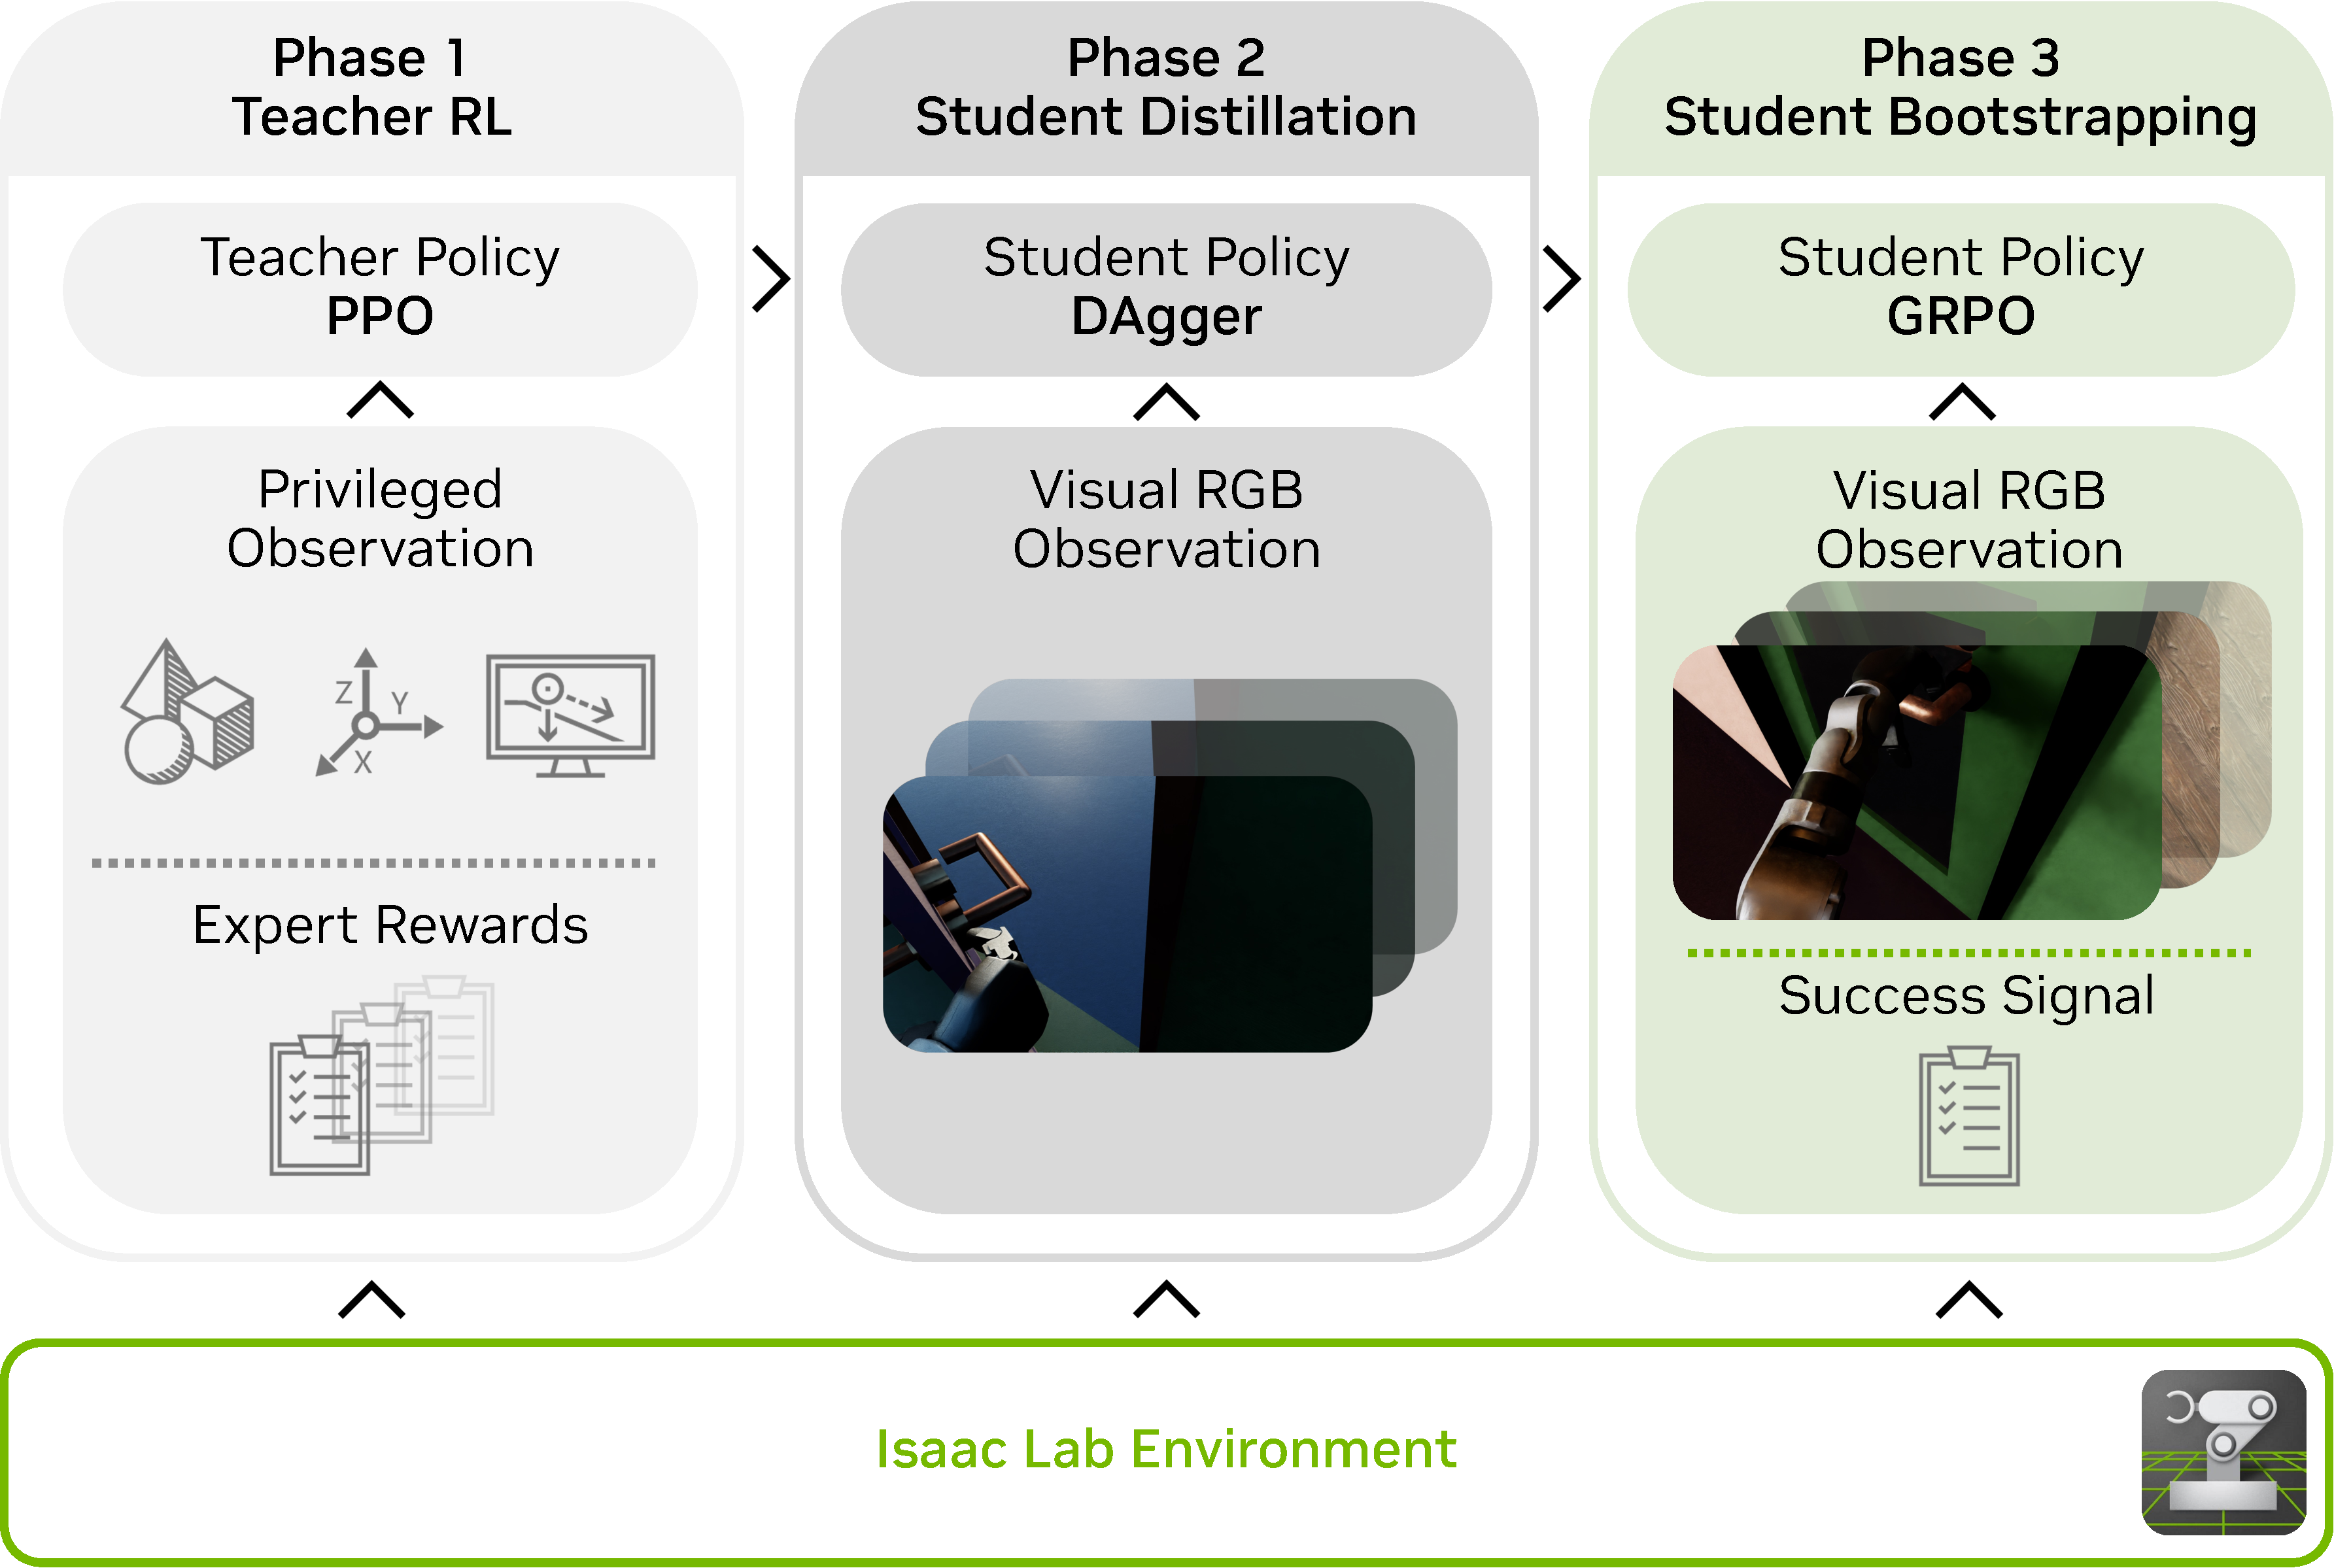
\includegraphics[width=0.7\linewidth]{figs/drafts/fig_method.pdf}
    \caption{\method{} training pipeline. All phases are done interactively with IsaacLab. In Phase 1, we train a teacher policy with privileged observations. In Phase 2, we distill it into an RGB student policy using DAgger. In Phase 3, we further train the student policy with GRPO using a binary success signal.}
    \label{fig:pipeline}
\end{figure}

To summarize, the main contributions of our work are:

\begin{itemize}
    \item We present one of the first humanoid sim-to-real policy capable of diverse articulated loco-manipulation from pure RGB perception.
    \item We introduce a teacher-student-bootstrap pipeline for whole-body loco-manipulation, including a stage-reset exploration mechanism for stable teacher training and GRPO-based fine-tuning to mitigate the student policy's partial observability.
    \item We provide a physically accurate and visually diverse synthetic-generation pipeline in IsaacLab for humanoid navigation with interactable doors, designed to scale in parallel and distributed RL workflows.
    \item We demonstrate a 31.7\% improvement over human teleoperation using the same whole-body controller, highlighting the potential of photorealistic simulation for scaling vision-based whole-body loco-manipulation learning.
\end{itemize}